\documentclass[
    a4paper,
    DIV=14,
    abstract=true,
    numbers=noenddot
]
{scrartcl}

\usepackage{
    amsmath,
    amssymb,
    amsthm,
    array,
    authblk,
    bm,
    dsfont, % for 1 vector or indicator function
    graphicx,
    mathtools,
    nicefrac,
    physics,
    tabularx,
    tcolorbox,
    todonotes,
    tikz,
    xcolor,
    float,
    subcaption,
}
\usepackage[shortlabels]{enumitem}

\usepackage[T1]{fontenc}

\usepackage[pdffitwindow=false,
    plainpages=false,
    pdfpagelabels=true,
    pdfpagemode=UseOutlines,
    pdfpagelayout=SinglePage,
    bookmarks=false,
    colorlinks=true,
    hyperfootnotes=false,
    linkcolor=blue,
    urlcolor=blue!30!black,
    citecolor=green!50!black]{hyperref}


\newtheorem{theorem}{Theorem}[section]
\newtheorem{proposition}[theorem]{Proposition}
\newtheorem{lemma}[theorem]{Lemma}
\newtheorem{corollary}[theorem]{Corollary}
\newtheorem{definition}[theorem]{Definition}

\theoremstyle{definition}
\newtheorem{example}[theorem]{Example}
\newtheorem{observation}{Observation}
\newtheorem{assumption}{Assumption}

\newtheorem{exercise}{Exercise}

\newtheorem*{hint}{Hint}

\newenvironment{exerciseandhint}[2]
{\begin{exercise} #1

    \emph{Hint: #2}}
    {\end{exercise}}

\newcommand{\red}[1]{{\color{red}#1}}
\newcommand{\td}{\todo[inline,color=green!40]}

\bibliographystyle{elsarticle-num}
\newcommand{\fk}[1]{\mathfrak{#1}}
\newcommand{\wh}[1]{\widehat{#1}}
\newcommand{\tl}[1]{\widetilde{#1}}

\newcommand{\br}[1]{\left\langle#1\right\rangle}
\newcommand{\set}[1]{\left\{#1\right\}}
\newcommand{\qp}[1]{\left(#1\right)}\newcommand{\qb}[1]{\left[#1\right]}
\newcommand{\qt}[1]{\left(#1\right)}
\newcommand{\Id}{\bm{I}}\renewcommand{\ker}{\rm{ker}}\newcommand{\supp}[1]{\bm{supp}(#1)}\renewcommand{\tr}[1]{\mathrm{tr}\left(#1\right)}
\renewcommand{\norm}[1]{\left\lVert #1 \right\rVert}\renewcommand{\abs}[1]{\left| #1 \right|}
\newcommand{\U}{}\renewcommand{\star}{*}
\renewcommand{\Im}{\bm{Im}}
\newcommand{\iso}{\xrightarrow{\sim}}
\renewcommand{\d}{\,\mathrm{d}}\newcommand{\dx}{\,\mathrm{d}x}
\newcommand{\dy}{\,\mathrm{d}y}
\newcommand\restr[2]{\left.#1\right|{#2}}
\newcommand{\rmm}[1]{\mathrm{#1}}
\newcommand{\mat}[1]{\begin{bmatrix}{#1}\end{bmatrix}}

\newcommand{\A}{\mathbb{A}}
\newcommand{\C}{\mathbb{C}}
\newcommand{\E}{\mathbb{E}}
\newcommand{\F}{\mathbb{F}}
\newcommand{\N}{\mathbb{N}}
\newcommand{\Q}{\mathbb{Q}}
\newcommand{\R}{\mathbb{R}}
\newcommand{\Z}{\mathbb{Z}}
\newcommand{\Aa}{\mathcal{A}}
\newcommand{\Bb}{\mathcal{B}}
\newcommand{\Cc}{\mathcal{C}}
\newcommand{\Dd}{\mathcal{D}}
\newcommand{\Ee}{\mathcal{E}}
\newcommand{\Ff}{\mathcal{F}}
\newcommand{\Gg}{\mathcal{G}}
\newcommand{\Hh}{\mathcal{H}}
\newcommand{\Kk}{\mathcal{K}}
\newcommand{\Ll}{\mathcal{L}}
\newcommand{\Mm}{\mathcal{M}}
\newcommand{\Nn}{\mathcal{N}}
\newcommand{\Oo}{\mathcal{O}}
\newcommand{\Pp}{\mathcal{P}}
\newcommand{\Qq}{\mathcal{Q}}
\newcommand{\Rr}{\mathcal{R}}
\newcommand{\Ss}{\mathcal{S}}
\newcommand{\Tt}{\mathcal{T}}
\newcommand{\Uu}{\mathcal{U}}
\newcommand{\Vv}{\mathcal{V}}
\newcommand{\Ww}{\mathcal{W}}
\newcommand{\Xx}{\mathcal{X}}
\newcommand{\Yy}{\mathcal{Y}}
\newcommand{\Zz}{\mathcal{Z}}

\begin{document}
\title{Title}
\author{Author Name}
\date{\today}
\maketitle
\section{Section Name}
Interesting stuff to talk about
\section{No model is complete}
Within the Bayesian framework we consider a collection of statements $A_ \theta$ parametrised by a collection of parameters $\theta \in \Omega$. Our goal is to reason as to the plausibility of each of these statements. To do so, we do as follows.
\begin{enumerate}
    \item \textbf{Events}. We first consider a collection of statements indexed by a parameter $\theta $ which we denote $\Ss = \set{A_\theta: \theta \in \Omega}$. The collection $\Ss $ must form a $\sigma $-algebra. In particular, the complement $\overline{A_\theta }$ of $A_\theta $ must belong to $\Ss $. Likewise the logical disjunction $A_{\theta _1}+ \cdots A_{\theta _n}$ must also belong to $\Ss $.
    \item \textbf{Observations}. We consider a collection of observations $y$ which we denote $\Yy $. These represent the outcome of some experiment.
    \item \textbf{Prior}.   We use ``all'' our prior information to determine the prior distribution $p(\theta )$ which represents our initial degree of belief in each of the statements $A_\theta $ .
    \item \textbf{Likelihood}.   We study the system in question to ``determine'' the likelihood $p(y| \theta )$ of making an observation $y$ conditional on $A_\theta$.
    \item \textbf{Posterior}.  We use Bayes' theorem to update our prior beliefs to obtain the posterior distribution $p(\theta |y)$ which ``fully'' represents the plausibility of $\theta $ given the observation $y$.
\end{enumerate}
The question is, is this possible? In fact it is not for the following reasons.
\begin{enumerate}
    \item \textbf{Can we define a prior?}  The first step is possible, however it requires that the statements we are considering to be logically exhaustive. For more complex models this is almost never the case. Essentially for the reason that any reasonable person must consider the possibility that the very model they are studying is incorrect.
    \item  \textbf{Can we define the likelihood?}.  The second step requires that given data $y$ we define  an assignation of the form
          \begin{align*}
              p(|y): \Ss & \longrightarrow  [0,\infty) \\
              A          & \longmapsto p(A|y),\end{align*}
          where $\Ss $ is the set of all possible statements. Within Kolmogorov's axioms of probability $\Ss $ is referred to as the $\sigma $-algebra of possible events. This requires that we know in advance all possible statements that could be made. This is not possible.

\end{enumerate}

Let us consider first a simple example
\begin{example}\label{coin}
    One of the most classical examples in statistical theories is that of coin flipping. In Bayesian inference the problem is often set-up as follows.

    A coin is flipped repeatedly and the sequence $(y_1,...,y_n) \in \set{0,1}^n$  of heads $1$  and tails $0$. We consider the statements $A_\theta = \set{\text{The coin has probability $\theta $ of landing heads}}$ parametrised by $\theta \in [0,1]$. We set a uniform prior $p(\theta )=1$ on $[0,1]$ and consider the likelihood
    \begin{align*}
        p(y_n|y_1,...,y_{n-1},\theta )= p(y_n|\theta )= \theta ^{y_n}(1-\theta )^{1-y_n}.
    \end{align*}
    The posterior is then given by
    \begin{align*}
        p(\theta |y_1,...,y_n) \propto \theta ^{\sum y_i}(1-\theta )^{n-\sum y_i}.
    \end{align*}
    It is my belief that no one would actually reason like this. Suppose for example that you observe after $n-1=10^6$ tosses the alternating sequence $(1,0,1,0,....,1,0)$  (admittedly this is a large number of tosses, but some kind of electronic simulation may be considered just as well). The posterior $p(\theta |y)$ is very sharply peaked around $\theta =1/2$ and as a result, the likelihood of the next toss is approximately uniform
    \begin{align*}
        p(y_{n}=1|y_1,...,y_{n-1})\approx 1/2, \quad p(y_{n}=0|y_1,...,y_{n-1})\approx 1/2.
    \end{align*}
    However, I'm inclined to believe that after such a sequence of tosses all but the most dogmatic would decide that the coin simply alternates between heads and tails and
    \begin{align*}
        p(y_n=1|y_1,...,y_{n-1})\approx 1.
    \end{align*}
\end{example}
What went wrong in \Cref{coin} is that we did not allow for any dependence of future throws on previous ones in the likelihood $p(y|\theta )$. As a result, the model of course could not take any into account. This issue can perhaps be resolved by considering a more complex model but this is not always clear how to do. Consider the following more abstract example common in Bayesian inverse problems.
\begin{example}
    Consider a function $G: \R^n \to \R^m $. We consider the model
    \begin{align*}
        y=G(u)+ \varepsilon,
    \end{align*}
    where the distribution  $(u,\varepsilon)$ depends on some parameter $\theta \in \Omega$. For example, $u$ might be a spatial Gaussian field with mean and covariance parametrised by  $\theta_1 \in \R^{n_1},$ and $\varepsilon$ is independent from $u$  with mean and covariance parametrised by $\theta _2 \in \R^{n_2}$ with $\theta =(\theta _1, \theta _2 )$, and $G$ is linear.

    The distribution on $u,\varepsilon $ determines the likelihood $p(y|u,\varepsilon )$ and once we define the prior $p(\theta )$ we can then (at least in principle) calculate the posterior $p(\theta |y)$.

    However, no matter what distribution is chosen for $u,\varepsilon $ and what function $F$ is considered , if one observes for some other reasonable function $F \neq G$, say $u=(u_1,....,u_n)\to (u_1^2,0,...,0)$,
    \begin{align*}
        y=F(u).
    \end{align*}
    Then one should strongly consider the possibility that the model is incorrect and rather it is $F$ that contains the true relationship between $y$ and $u$. This is not possible within the Bayesian framework as the model, once chosen, is fixed and admits no changes.

    One could try to remedy the above problem by considering $G$ to live in some space of admissible functions $ \Hh $ and set a prior $p(G)$ on $\Hh$. However, what space of functions can be chosen? It is my belief that whatever $\Hh $  is chosen one could be persuaded that $G$ is not in $\Hh $ and that the model is incorrect. For example one could take $\Hh $ to be the space of functions of some regularity, say $\Hh = H^s(\R^n)$. But then what if one observed a non-smooth relationship such as $y=F(u)$ with $F= \delta _0$. Would one still consider the model to be correct with probability $1$?
\end{example}
I hope that the above examples show that
\begin{itemize}
    \item Bayesian inference depends on a fixed model being defined and operates within the confines of this model.
    \item No matter what model is chosen, one  always consider the possibility that the model is incorrect. This is outside the scope of the model and of Bayesian inference.
\end{itemize}
The above is somewhat resonates somewhat with Godel's incompleteness theorem. In the same way that no formal system can be both consistent and complete, no model can be both correct and complete. This is not to say that Bayesian inference is not useful, but rather that it is not the be all and end all of statistical reasoning. In the same way that Godel's theorem does not mean that mathematics is useless, but rather that it is not the be all and end all of reasoning.

\section{Is Bayesian inference a mirror for scientific reasoning?}

Though incomplete, as Cox's theorems \cite{van2003constructing} shows, Bayesian inference is the only way of reasoning in the face of consistency that respects basic desiderata and introduce probability as the only valid principles of logic without referring to chance or random variables.

The situations described above are well known to the physicist, a theory is never complete and one must always consider the possibility that the theory is incorrect. However, despite this constant state of incorrectness, physics and science as a whole still makes remarkable progress. Why?

In Bayesian inference probability is introduced as a extended logic in the presence of incomplete information. This is exactly the situation in science. In this sense, Bayesian inference is a mirror for scientific reasoning. However, the Bayesian framework is not enough to explain why science works. In the following sections we will discuss why this is the case and what is needed to explain why science works.


Let us write $M= \sum_{\theta \in \Omega } A_\theta $ for the statement that one of the statements $A_\theta $ is true and consider the logical negation $\overline{M}= \prod_{\theta }\overline{A_\theta}$. By considering $\overline{M}$ we allow for the fact that we are wrong, something that is necessary in any reasonable model. To compare the plausibility of $M$ and $\overline{M}$ we can consider the ratio
\begin{equation}
    \frac{p(M|y)}{p(\overline{M}|y)}= \frac{p(M)p(y|M)}{p(\overline{M})p(y|\overline{M})}.
\end{equation}
This requires that we define the prior $p(M)$ and $p(\overline{M})$. If one had no strong prior information (however I would argue that in fact $p(M)=0$ and perhaps it is better to compare which model is better), in the interest of fairness one could consider $p(M)=p(\overline{M})=1/2$.The likelihood $p(y|M)$ is determined by the already defined likelihood $p(y|\theta )$ and prior $p(\theta|M)=  p(\theta )$ as
\begin{align*}
    p(y|M) & = \int_{\Omega } p(y|\theta )p(\theta)\d \theta.
\end{align*}
To determine the likelihood $p(y|\overline{M})$. If we are given no further information the only reasonable choice is, by the principle of indifference, to assign a uniform distribution. However, if $\Yy $ is unbounded this is not possible and we reach an impasse.


However this still does not completely solve the problem. For example.
\section{Judging the quality of a model}
There are two option
\begin{enumerate}
    \item \textbf{Is the model better than the alternatives?}  Though no model is perfect some models are better than others. To check whether a model is better than another we can stay within the Bayesian Framework and use model selection. This only requires we set a prior distribution for models $M_j$ and then calculate the posterior distribution $p(M_j|y)$ for each model. The model with the highest posterior probability is then the model we are most confident of. That is, the best model.
    \item \textbf{Is the model useful?} To answer this question we need to study ``how wrong'' the model is.  To quote George Box, ``All models are wrong, but some are useful''. How can we determine whether a model is useful? To do so we need to leave the confines of Bayesian inference. This is because Bayesian inference operates within the premise that the model considered is correct and therefore it does not make sense to study how wrong the model is. We will study this question later and define posterior predictive checks.
\end{enumerate}
\section{Why does science work?}
The question is, if every model is false, why can we draw useful conclusions from them.
This questions is relevant for Bayesian inference as well. As we have seen above, the Bayesian framework also requires the specification of an approximative model. The output of the Bayesian analysis is a posterior distribution which reflects the plausibility we assign to each statement of our model.

Believing that reality adheres to these probabilities through some kind of long term frequency or ``law of large numbers'' is the frequentist assumption and is said to be a case of the mind projection fallacy by Jaynes. Jaynes defines this as the belief that ``one’s own private thoughts and sensations are realities existing externally in Nature''. However, I would argue that science, and Bayesian inference, to some extent requires this projection. To be more concrete, Bayesian theory defines the probability  $p(A)$ of a statement $A$  as \emph{a state of knowledge that represents the degree of plausibility of $A$} and not as a physical property of the universe. The claim is that, as a result, we have no right to believe that the universe must agree with any of our probabilities.  Though I agree, the very definition of the probability $p(A)$  requires that, for $p(A) \neq 0$  we have some plausibility to $A$. In particular, if we are almost certain about $A$ so $p(A)$ is close one, but we observe that $A$ is false are we not surprised? If we are surprised, is it not because we expected reality to conform to statement $A$?

Furthermore, in practice, we use these probabilities to make predictions about the future and to make decisions and it is indisputable that acting on reality through the plausibility of a model is often a useful strategy. But if reality is unrelated to our belief in it why is this the case? This is the question we will try to answer in the following sections.
\subsection{Good models from a scientific perspective}
A physical model typically predicts the outcome $y$ of some experiment $E$ with state $\theta _E$. That is, it is concerned with relationships of the form $y=G(\theta _E)$ for some function $G$. In reality, we know that every model is approximate and no physical theory can claim to be exact. So rather the goal is a relationship of the form
\begin{align*}
    y\approx G(\theta _E).
\end{align*}
We now suppose that there is a true relationship that may depend on more parameters than the model $G$ allows. That is, there is a true relationship of the form
\begin{align*}
    y= F(\theta _E, \eta_E).
\end{align*}
This corresponds to the assumption that
\begin{itemize}
    \item The object we are talking about exists. It is not a figment of our imagination.
    \item The universe is deterministic and given the initial conditions $(\theta _E, \eta_E)$ the outcome of the experiment is determined. Here $\eta _E$ may be arbitrarily large so that no physical theory can capture it in practice. For example it may contain the position of every particle in the universe or any other quantities.
\end{itemize}



Given a metric $d$ on the space of outcomes $\Yy $ we can define how close our model is for any given experiment $E$
\begin{definition}
    Consider a model $G(\theta )$ and an experiment $E =(\theta_E,\eta_E)$. Write $y_{\text{model}}:= G(\theta_E)$ and $y_{\text{true}}:= F(\theta_E, \eta_E)$.     We say that $G$ is an \emph{$\varepsilon $ approximation of reality for experiment $E$} if
    \begin{align*}
        d(y_{\text{approx} },y_{\text{true} })< \varepsilon.
    \end{align*}
\end{definition}
The size of $\varepsilon $ is the precision of the model and an acceptable accuracy will depend on what is being measured, for example, we may be willing to tolerate smaller accuracy in the measurement of the orbit of a planet around the sun than that of an electron around a nucleus. In theory, there is no reason to expect that we can find a model that is a close approximation for reality. In fact, it is a remarkable fact that science is able to do so at the scale of subatomic particles. To quote Einstein, ``The eternal mystery of the world is its comprehensibility… The fact that it is comprehensible is a miracle.''

In practice, we may be interested not with any one experiment but a collection of experiments $\Ee $
\begin{definition}
    Let $\Ee $ be a collection of experiments, then we say that $G$ is an \emph{$\varepsilon $ approximation of reality for $\mathcal{E}$} if it is an $\varepsilon $ approximation of reality for every experiment $E \in \mathcal{E} $.
\end{definition}
It is unreasonable to suppose that the model will perform well for every experiment. For example, a model for the trajectory of a ball using only the initial position and velocity will lose all accuracy if we exert a large external force on the ball (for example by hitting it with a bat).

\subsection{Good models from a Bayesian perspective}
In the Bayesian framework our model now takes on a probabilistic flavour. We now have our likelihood and prior
\begin{align*}
    p(y|\theta ), \quad p(\theta ).
\end{align*}
Now we must ask what does it mean for this model to be a good representation of reality.
From a strictly Bayesian standpoint this question does not make sense as the likelihood only reflects a state of mind and to assume that reality actually conforms to this is the mind projection fallacy. As a result, it is necessary to move outside of the Bayesian framework to answer this question.
\subsubsection{The inverse problem}
If our Bayesian model is to be applied, we must first ``train it'' by observing some experiment $E$. Let us write $y= \tl{F}(\theta_E, \eta _E)$ for the outcome of the experiment $E$. We note that our observation is not necessarily the true outcome $y=F(\theta _E, \eta _E)$ as our measurement may be imprecise. However, it is a deterministic function of the state of our experiment.

Having observed $y$ we can calculate the posterior distribution $p(\theta |y)$ which reflects our updated beliefs about the state of the experiment. However, as our model is approximate and, at least theoretically, calculate the distance between the true state of the experiment and the posterior distribution
\begin{definition}
    Consider an experiment $E$ with state $(\theta _E$, $\eta _E)$. Write $y$ for the observation of the experiment. Then, we say that a Bayesian model $p(y|\theta )$ is an \emph{$\varepsilon $ approximation of reality for hte inverse problem under experiment $E$} if
    \begin{align*}
        S(p(\theta  |y), \theta _E)< \varepsilon.
    \end{align*}
\end{definition}
Here, $S$ is a \emph{score function} which measures the distance between the posterior distribution and the true state of the experiment. The choice of $S$ will depend on the nature of the experiment and the state of the experiment.

What properties should $S$ have? Bayesian theory can say nothing about this as it lies outside of the Bayesian framework. However, we can make some reasonable assumptions.
Suppose for example that we were presented with a sequence of experiments $E_n$ in such a way that $\theta _{E_n}$ appears distributed according to some distribution $q(\theta )$. That is, for all continuous and bounded functions $f$ we have
\begin{align}\label{distribution limit}
    \lim_{n\to\infty}\E\qb{ f(\theta _{E_n})}= \int f(\theta )q(\theta )\d \theta.
\end{align}
This is an idealized situation and cannot occur in practice as we will never observe an infinite amount of experiments. However, it is convenient mathematically and more practically we can consider that we observe a large number of experiments such that the expression in \eqref{distribution limit} is approximately true.

This state of events would correspond to the setting where $\theta$ appears to be ``random'' with distribution $q$. Then, the best we could hope for our posterior probability is that it is close to the ``true distribution'' $q$ that is. The minimum of $S$ should occur when $p(\theta |y)=q(\theta )$. This leads to the following definition
\begin{definition}
    We say that a score function $S$ is \emph{proper} if
    \begin{align*}
        S(p(\theta |y), \theta _E)=0 \iff p(\theta |y)=q(\theta ).
    \end{align*}
\end{definition}


\begin{definition}
    Consider an experiment $E$ with state $(\theta _E$, $\eta _E)$.
    Write $y'$ for the outcome of a new experiment $E'$ with state $\theta _{E'}$.
    We say that a Bayesian model $p(y|\theta )$ is an \emph{$\varepsilon $ approximation of reality for experiment $E$} if
    \begin{align*}
        S(p(y'|y),y)< \varepsilon,
    \end{align*}

\end{definition}
\section{Can a theory ever be proved true?}
Suppose that we wish to prove some theory. To do so, we must use the information we have available and some logical steps to arrive at the conclusion that the theory is true. However, all the information we have is sensory. That is, we do not possess any information that we do not receive through our senses, be this a reading of a thermometer or the observation of a star through a telescope. Unfortunately, our senses are not perfect and are subject to error. We may think the thermometer says $30$ degrees, but however unlikely it may be, we may have misread it, hallucinated or any other number of possibilities. As a result, we can never be certain that the information we have is correct and as a result, we can never be certain that the theory we have proved is true. Jaynes argues to the contrary that some theories can be proved true and says the following
``a simple counter-example to a principle sometimes stated by philosophers, that theories cannot be proved true, only false. We seem to have just the opposite situation for the theory that there was once life on Mars. To prove it false, it would
not suffice to dig up every square foot of the surface of Mars; to prove it true one needs only to find a single fossil.'' However, he obviates the fact that we may think we have discovered a fossil, but we can never be sure.

On a similar note, we also disagree that a theory can be proven false, as to do so, we once more reason based on our uncertain sensory information and as a result cannot ever be convinced that we are right in proving the theory false. We can only reason as to the truth or falsity of such events with high probability, but never absolute certainty.

\section{Is interpreting probability as subjective belief sufficient?}
In the Bayesian interpretation, a probability is a state of mind that represents the degree of plausibility of a statement. It is subjective and need have no relation to the physical world. As a result, it makes no sense to say whether a probability assignment is good or bad. However, in my view this is the point of probabilities is that they serve as a model for the physical world. If they do not do this, then they are useless.

Consider the following example. A certain news outlet reports on sports matches, and are in the habit of assigning probabilities to each possible outcome before the match. After one year of this, a large amount of predictions have been made and the outcomes recorded. If events happen roughly as often as predicted you and I would be inclined to believe that the probabilities assigned are good. If not, say that teams that were predicted to win 90\% of the time only win 10\% of the time, then we would be inclined to believe that the probabilities assigned are bad. However, the news outlet is well versed in Bayesian epistemology and would argue that the probabilities they assign are subjective and as a result cannot be good or bad. Any attempt by us to evaluate their predictions is a gross overreach.
\begin{figure}[htbp]
    \centering
    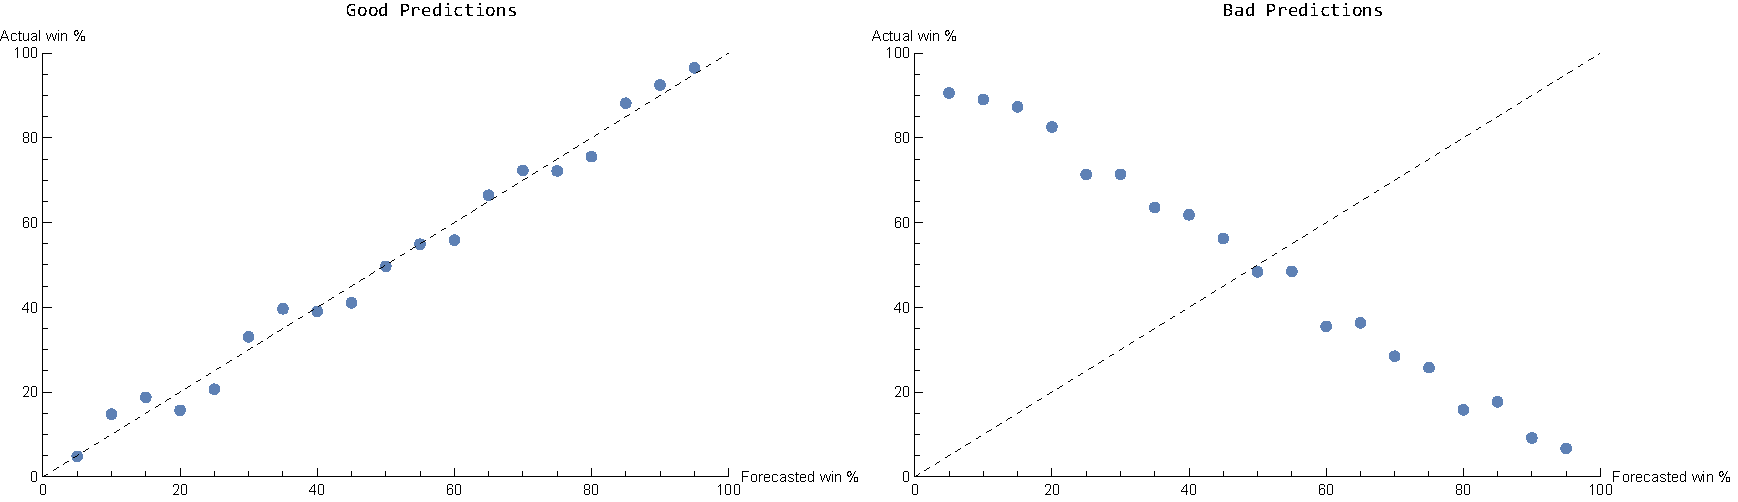
\includegraphics[width=\textwidth]{calibration_plots.pdf}
    \caption{Calibration plots for a news outlet. The x-axis represents the predicted probability of an event and the y-axis the actual frequency of the event. The diagonal line represents perfect calibration. The left plot shows that the news outlet is well calibrated, the right plot shows that the news outlet is poorly calibrated.}
    \label{fig:}
\end{figure}

It is my belief that this is a misunderstanding of the Bayesian framework should strive to be. The probabilities assigned by the news outlet though subjective, should be good in the sense that they are a good model for reality. If they are not, then they are useless. In the next section, we will discuss what it means for a model to be a good model, how we can evaluate this and how this enriches the Bayesian framework.




\bibliography{biblio.bib}

\end{document}